\section{Winding Numbers and Cauchy's Integral Formula}

\begin{lemma}\label{4.5.1}
    Let $\y:[0,1] \xrightarrow{} \C$ be a closed rectifiable path. Define, for
    $z_0 \notin \{\y\}$ the path integral
    \begin{equation*}
        W=\frac{1}{2i\pi}\int_\y{\frac{dz}{z-z_0}}
    \end{equation*}
    Then $W \in \Z$.
\end{lemma}
\begin{proof}
    Suppose, without loss of generality, that $\y$ is of class  $C^1$. Define
    $g:[0,1] \xrightarrow{} \C$ by
    \begin{equation*}
        g(t)=\int_0^t{\frac{\y'(s)}{\y(s)-z_0} \ ds}
    \end{equation*}
    hence $g(0)=0$ and $g(1)=\int_\y{\frac{dz}{z-z_0}}$. Moreover, notice that
    \begin{equation*}
        g'(t)=\frac{\y'(s)}{\y(s)-z_0} \text{ on } 0 \leq t \leq 2\pi
    \end{equation*}
    Then we get $D{(\exp{(-g)(\y-z_0)})}=0$ so that $\exp{(-g)(\y-z_0)}$ is the
    constant function, and
    $\exp{(-g)(\y(0)-z_0)}=\exp{(-g)(\y(1)-z_0)}=2i\pi{k}$, and $k \in \Z$.
    Notice that $k$ is precisely $W$.
\end{proof}

\begin{definition}
    Let $\y$ be a rectifiable closed path in  $\C$. We define the
    \textbf{winding number} of $\y$  \textbf{around} some point $z_0 \notin
    \{\y\}$ to be the path integral given by
    \begin{equation*}
        W(\y,z_0)=\frac{1}{2i\pi}\int_\y{\frac{dz}{z-z_0}}
    \end{equation*}
\end{definition}

\begin{lemma}\label{4.5.2}
    If $\y$ and $\s$ be closed rectifiable paths having the same initial points.
    Then the following are true
    \begin{enumerate}
        \item[(1)] $W(\y,z_0)=-W(\y^-,z_0)$ for all $z_0 \notin \{\y\}$.

        \item[(2)] $W(\y+\s,z_0)=W(\y,z_0)+W(\s,z_0)$ for all $z_0 \notin \{y\}
            \cup \{\s\}$.
    \end{enumerate}
\end{lemma}

\begin{definition}
    Let $\y$ be a closed path. We define the \textbf{interior} of $\y$ to be the
    open set  $U$ of $\C$ having as boundry the trace  of $\y$, i.e.
    $\partial{U}=\{\y\}$. We denote the interior of $\y$ by $\Int{\y}$. We call
    an open set $U$ of the set $\com{\C}{\{\y\}}$ a component \textbf{bounded}
    by $\y$ if $U \subseteq \Int{\y}$, and \textbf{unbounded} otherwise.
\end{definition}

\begin{figure}[h]
    \centering
    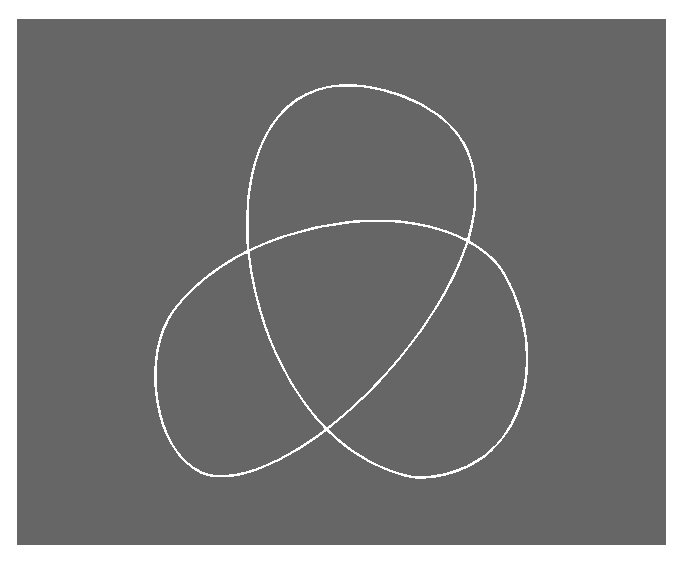
\includegraphics[scale=0.5]{Figures/Chapter4/bounded_components.eps}
    \caption{A closed rectifiable path $\y$ (removed from $\C$) with its
        bounded components. Notice that the component lying outside of
    $\{\y\}$ is an unbounded component.}
    \label{fugure_4.2}
\end{figure}

\begin{theorem}\label{4.5.3}
    Let $\y$ be a closed rectifiable path in  $\C$. Then  $W(\y,z_0)$ is
    constant for any $z_0$ in a component $U$ of  $\com{\C}{\{\y\}}$. Moreover,
    if $z_0$ is in an unbounded component, then  $W(\y,z_0)=0$.
\end{theorem}
\begin{proof}
    Let $f:U \xrightarrow{} \C$ be defined by $f(z)=W(\y,z)$. Now, fix a $z_0
    \in U$, and let $r$ be the distance between  $z_0$ and $\{\y\}$. If
    $|a-b|<\d<\frac{r}{2}$, then we  get
    \begin{equation*}
        |f(a)-f(b)|=
        \frac{1}{2i\pi}\Big{|} \int_\y{\frac{a-b}{(z-a)(z-b)} \ dz} \Big{|} \leq
        \frac{|a-b|}{2i\pi}\int_\y{\frac{|dz|}{|z-a||z-b|}}
    \end{equation*}
    now, for $|a-b|<\frac{r}{2}$, and $z \in \{\y\}$, we get $|z-a| \leq
    r>\frac{r}{2}$, thus $|f(a)-f(b)|<\frac{2\d}{\pi{r^2}}V(\y)$ so if $\e>0$,
    choosing  $\d<\min{\{\frac{r}{2}, \frac{\pi{r^2}}{2V(\y)}\}}$, and we get
    that $f$ is continuous.

    Now, if $U$ is a component of $\com{\C}{\{\y\}}$, then $f(U)$ is connected.
    However, notice that $f(U) \subseteq \Z$, so that $f(U)$ must be pointset.
    Therefore $f$ is constant on $U$.

    Now, let $V$ be an unbounded component of $\com{\C}{\{\y\}}$; i.e. $V
    \notsubseteq \int{\y}$; then there exists an $R>0$ such that the set  $\{z
    \in V : |z|>R\} \subseteq V$. If $\e>0$, choose a point  $z_0$ with
    $|z_0|>R$, and $|z-z_0|>\frac{V(\y)}{2\pi\e}$ uniformly for $z \in
    \{\y\}$. Then $|W(\y,z_0)|<\e$ so that $W(\y,z_0) \xrightarrow{} 0$. Since
    $W(\y,z_0)$ is constant, this makes $W(\y,z_0)=0$ on $V$.
\end{proof}

\begin{lemma}\label{4.5.4}
    LEt $\y$ be a rectifiable path, and let  $\phi$ be a continuous function on
     $\y$. Define
     \begin{equation*}
         F_m(z)=\int_\y{\frac{\phi(w)}{(w-z)^m} \ dw}
     \end{equation*}
     for every $z \notin \{\y\}$. Then each $F_m$ is analytic on
     $\com{\C}{\{\y\}}$, and
     \begin{equation*}
         F_m'(z)=mF_{m+1}(z)
     \end{equation*}
\end{lemma}
\begin{proof}
    Notice that since $\{\y\}$ is compact, $\y$ is bounded, and hence we get
    \begin{equation*}
        \frac{1}{(w-z)^m}-\frac{1}{(w_0z_0)^m}=
        (z-z_0)\sum_{i=0}^{\infty}{\frac{1}{(w-z)^{m-i}(w-z_0)^i}}
    \end{equation*}
    This makes the function $F_m$ continuous.

    Now, fix $z_0 \in \com{\C}{\{\y\}}$, and let $z \in \com{\C}{\{\y\}}$, whith
    $z \neq z_0$. Then it follows that
    \begin{equation*}
        \frac{F_m(z)-F_m(z_0)}{z-z_0}=\int_\y{\frac{\phi(w)}{(w-z)^m(w-z_0)} \
        dw}+\dots+\int_\y{\frac{\phi(w)}{(w-z)(w-z_0)^m} \ dw}
    \end{equation*}
    now, since $z_0 \notin \{\y\}$,
    \begin{equation*}
        \frac{\phi(w)}{(w-z_0)^k}
    \end{equation*}
    is continuous on $\{\y\}$ for every $k$. Then each integral defines a
    continuous function of  $z \in \com{\C}{\{\y\}}$. Taking $z \xrightarrow{}
    z_0$, this limit exists and gives us
    \begin{equation*}
        F_m'(z_0)=m\int_\y{\frac{\phi(w)}{(w-z_0)^{m+1}} \ dw}=mF_m(z_0)
    \end{equation*}
\end{proof}

\begin{theorem}[Cauchy's Integral Formula]\label{4.5.5}
    Let $U$ be an open set of  $\C$, and  $f:U \xrightarrow{} \C$ an analytic
    function. If $\y$ is a closed rectifiable path in  $U$, with  $W(\y,w)=0$,
    for every $w \in \com{\C}{U}$, then for every $z_0 \in \com{\C}{\{\y\}}$,
    \begin{equation*}
        W(\y,z_0)f(z_0)=\frac{1}{2i\pi}\int_\y{\frac{f(z)}{z-z_0} \ dz}
    \end{equation*}
\end{theorem}
\begin{proof}
    Define $\phi:U \times U \xrightarrow{} \C$ by
    \begin{equation*}
        \phi(z,w)=\frac{f(z)-f(w)}{z-w}
    \end{equation*}
    if $z \neq w$, and $\phi(z,z)=f'(z)$. Then $\phi$ is continuous on  $U
    \times U$, and moreover, $\phi$ is analytic on $U \times U$. Now, let
    $H=\{w \in \C : W(\y,w)=0\}$. Since $W(\y,w)$ is continuous, and defined on
    $\Z$,  $H$ is open. Moreover, we observe that  $H \cup U=\C$.

    Now, define the complex valued function $g:\C \xrightarrow{} \C$ by
    \begin{equation*}
        g(z)=\int_\y{\phi(z,w) \ dw} \text{ if } z \in U
    \end{equation*}
    and
   \begin{equation*}
       g(z)=\int_\y{\frac{f(w)}{z-w} \ dw} \text{ if } z \in H
   \end{equation*}
   Then for every $z \in H \cap U$, we get
   \begin{equation*}
        \int_\y{\phi(z,w) \ dw}=\int_\y{\frac{f(w)}{z-w}
   \end{equation*}
   so that
   \begin{equation*}
       \int_\y{\frac{f(w)}{z-w} \ dw}-f(z)W(\y,z)2i\pi=0
   \end{equation*}
   This makes $g$ well defined.

   Now, by the lemma \ref{4.5.4}, $g$ is analytic on  $H$, and by an analog to
   Leibniz's rule,  $g$ is analytic on  $U$. This makes  $g$ analytic on  $H
   \cup U=\C$; i.e. entire. Now, by definition,  $H$ is an unbounded component
   of  $\y$, and contains a neighborhood of  $\infty$ in $\C_\infty$ . Since $f$
   is bounded on  $\{\y\}$ and $\frac{1}{z-w} \xrightarrow{\text{uniformly}} 0$
   as $z \xrightarrow{} \infty$ for all $w \in \{\y\}$, we get
   \begin{equation*}
       \lim_{z \xrightarrow{} \infty}{g(z)}=
       \lim_{z \xrightarrow{} \infty}{\int_\y{\frac{f(w)}{w-z} \ dw}}=0
   \end{equation*}
   In particular, there is an $R>0$ such that  $|g(z)| \leq 1$ for every $|z|
   \geq R$. Since  $g$ is bounded on the closed ball $\bar{B}(0,R)$, $g$ is a
   bounded entire function. Therefore, by Liouville's theorem,  $g$ is constant.
   Hence  $g(z)=0$ for every $z \in \C$, so for  $z_0 \in \com{U}{\{\y\}}$, we
   get
   \begin{equation*}
       \int_\y{\frac{f(z)}{z-z_0} \ dw}-f(z_0)W(\y,z_0)2i\pi=0
   \end{equation*}
\end{proof}
\begin{corollary}
    If $\y_1, \dots, \y_m$ are closed rectifibale paths in $U$ such that
    $\sum{W(\y_k,w)}=0$ for every $w \in \com{\C}{U}$ and $1 \leq k \leq m$,
    then for every $z_0 \in \com{U}{\bigcup{\y_i}}$, we have
    \begin{equation*}
        f(z_0)\sum_{i=1}^m{w(\y_k,z_0)}=
        \sum_{i=1}^m{\frac{1}{2i\pi}\int_{\y_k}{\frac{f(Z)}{z-z_0}} \ dz}
    \end{equation*}
\end{corollary}

\begin{example}\label{exmaple_4.4}
    Let $U=\{z \in \C : R_1<|z|<R_2\}$ and define the paths $\y_1$ and $\y_2$ in
    $U$ by
    \begin{align*}
        \y_1(t) &=  r_1e^{it} \text{ on } 0 \leq t \leq 2\pi    \\
        \y_2(t) &=  r_2e^{-it} \text{ on } 0 \leq t \leq 2\pi    \\
    \end{align*}
    with $R_1<r_1<r_2<R_2$. Then if $|w|<R_1$, we have $W(\y_1,w)=1=-W(\y_2,w)$.
    If $|w| \geq R$, then  $W(\y_1,w)=W(\y_2,w)=0$. So that we have
    $W(\y_1w)+W(\y_2,w)=0$ for all $w \in \com{\C}{U}$.
\end{example}

\begin{theorem}\label{4.5.6}
    Let $U$ be open in  $\C$ and  $f:U \xrightarrow{} \C$ analytic. If $\y_1,
    \dots, \y_m$ are closed rectifiable paths in $\C$, such that
    $\sum{W(\y_k,w)}=0$ for all $w \in \com{\C}{U}$, then for every $z_0 \in
    \com{U}{\bigcup{\{\y_k\}}}$, and $k \geq 1$, we have
    \begin{equation*}
        f^{(k)}(z_0)\sum_{k=1}^m{W(\y_k,z_0)}=
        k!\sum_{k=1}^m{\frac{1}{2i\pi}\int_{\y_k}{\frac{f(z)}{(z-z_0)^k+1} \ dz}}
    \end{equation*}
\end{theorem}
\begin{corollary}
    If $\y$ is a closed rectifiable path in  $U$ with  $W(\y,w)=0$ for ever $w
    \in \com{\C}{U}$, then for every $z_0 \in \com{U}{\{\y\}}$, we have
    \begin{equation*}
        f^{(k)}(z_0)W(\y,z_0)=
        \frac{k!}{2i\pi}\int_\y{\frac{f(z)}{(z-z_0)^{k+1}} \ dz}
    \end{equation*}
\end{corollary}

\begin{definition}
    We call a closed path \textbf{triangular} if it is a polygonal path defining
    a triangle; i.e. a polygonal path with three sides.
\end{definition}

\begin{theorem}[Morera's Theorem]\label{4.5.7}
    Let $U$ be a region in $\C$, and let  $f:U \xrightarrow{} \C$ be a continuous
    complex valued function such that $\int_T{f}=0$ for every triangular path
    $T$, Then  $f$ is holomorphic on $U$.
\end{theorem}
\begin{proof}
    Suppose, without loss of generality, that $U$ is an open ball  $U=B(z_0,R)$
    of radius $R>0$ centered about a point $z_0 \in \C$. Now, for each $z \in
    U$, define
    \begin{equation*}
        F(z)=\int_{[z_0,z]}{f}
    \end{equation*}
    Now, fix $w_0 \in U$, then for every $z \in U$, we get
    \begin{equation*}
        F(z)=\int_{[z_0,w_0]}{f}+\int_{[w_0,z]}{f}
    \end{equation*}
    hence
    \begin{equation*}
        \frac{F(z)-F(w_0)}{z-w_0}=\int_{[w_0,z]}{f}
    \end{equation*}
    hence
    \begin{equation*}
        \frac{F(z)-F(w_0)}{z-w_0}-f(w_0)=
        \frac{1}{z-w_0}\int_{[w_0,z]}{(f(w)-f(w_0)) \ dw}
    \end{equation*}
    taking abosulte values gives us
    \begin{equation*}
        \Big{|}\frac{F(z)-F(w_0)}{z-w_0}-f(w_0)\Big{|} \leq
        \sup_{w \in [w_0,z]}{\{|f(w)-f(w_0)|\}}
    \end{equation*}
    so that
    \begin{equation*}
        \lim_{z \xrightarrow{} w_0}{\frac{F(z)-F(w_0)}{z-w_0}}=f(w_0)
    \end{equation*}
\end{proof}
